\documentclass{beamer}
\usetheme{}
\usecolortheme{dolphin}           
\useinnertheme{circles}
\setbeamertemplate{itemize items}[default]
\setbeamertemplate{enumerate items}[default]
\usepackage[T1]{fontenc}
\usepackage[utf8]{inputenc}
\usepackage{lmodern}
\usepackage{amsmath}
\usepackage{booktabs} 
\usepackage{graphicx}        
\usepackage{array}
\usepackage{color}
\makeatletter
\def\zapcolorreset{\let\reset@color\relax\ignorespaces}
\def\colorrows#1{\noalign{\aftergroup\zapcolorreset#1}\ignorespaces}
\makeatother
\setbeamertemplate{navigation symbols}{}
\setbeamertemplate{footline}[frame number]

%--------------------------------------
\title{Optimum currency areas}
\author{School of Economics, University College Dublin}
\date{Spring 2018}
\begin{document}

%--------------------------------------
\begin{frame}
 \titlepage
\end{frame}
%--------------------------------------

%--------------------------------------
\begin{frame}
  \begin{figure}
    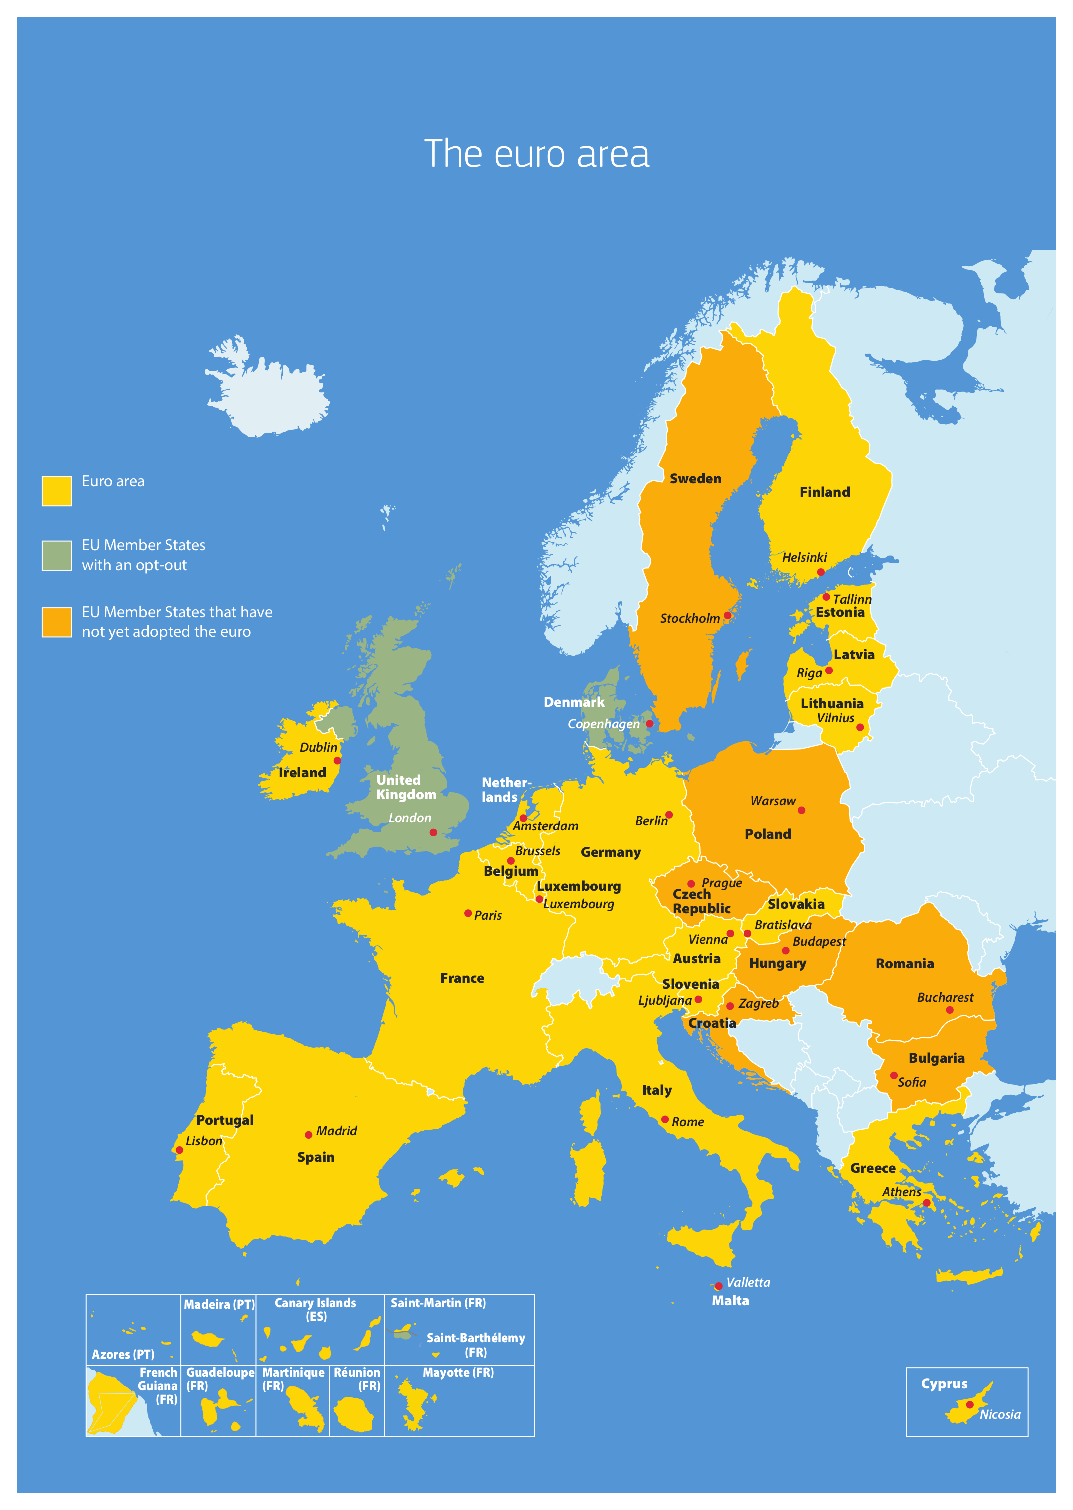
\includegraphics[scale=.3]{eurozone.eps}
  \end{figure}
\end{frame}
%--------------------------------------

%--------------------------------------
\begin{frame}
  \textbf{The Euro} according to the EU
  \begin{quote}
    The euro is the most tangible proof of European integration – the common currency in 19 out of 28 EU countries and used by some 338.6 million people every day. The benefits of the common currency are immediately obvious to anyone travelling abroad or shopping online on websites based in another EU country.
  \end{quote}
  \medskip
  \begin{itemize}
    \item Launched in 1999
    \item Replaced 12 national currencies in 2002
    \item Currently used by 19 of 28 member states
    \begin{itemize}
      \item 4 microstates adopted the Euro, and two state adopted currency unilaterally
    \end{itemize}
  \end{itemize}
\end{frame}
%--------------------------------------

%--------------------------------------
\begin{frame}
  \textbf{Brief history of European monetary integration}\\
  \medskip
  19th century-1944: Gold-standard \\
  1944 - 1971: Bretton-Woods system\\
  1970: Werner report\\
  1972: Snake in the tunnel\\
  1979: European Monetary System\\
  1992: Economic and Monetary Union\\
  2002 - present: Euro  
\end{frame}
%--------------------------------------

%--------------------------------------
\begin{frame}

\end{frame}
%--------------------------------------

%--------------------------------------
\begin{frame}
  \textbf{Mundell} (1961), "A Theory of Optimum Currency Areas"
  \medskip
  \begin{enumerate}
    \item Can a system of flexible exchange rates work effectively and efficiently in the modern world economy?   
    \begin{itemize}
       \item Involves lot of conditions for stability
       \item e.g. accounting for speculation; monetary discipline; debtors/creditors protection, etc.
     \end{itemize} 
    \item How should the world be divided into currency areas?    
  \end{enumerate}
  \medskip
  Can divide world into regions
  \begin{itemize}
     \item Within there is factor mobility
     \item Between there is factor immobility
   \end{itemize} 
   \medskip
  Region is an economic unit, but currency domain partly expression of national sovereignty.
\end{frame}
%--------------------------------------


%--------------------------------------
\begin{frame}
  \textbf{Benefits} of common currency area
  \begin{enumerate}
    \item Lowering of transaction costs
    \item Price transparency
    \item Uncertainty reduction
    \item Improvements in trade
    \item Quality of monetary policy
  \end{enumerate}
\end{frame}
%--------------------------------------

%--------------------------------------
\begin{frame}
  \textbf{Lowering of transaction costs}\\
  \begin{enumerate}
    \item Common currency means that there is no need to discuss currency of transaction
    \item Elimination of exchange rate
  \end{enumerate}
  2 implies that there is no loss in value. 
  \begin{itemize}
    \item Changing from currency to currency can lead to 50\% loss
  \end{itemize}
  \medskip
  Additionally, lowering of costs might increase competition  
\end{frame}
%--------------------------------------

%--------------------------------------
\begin{frame}
  \textbf{Price transparency}: prices are directly comparable across regions
  \begin{enumerate}
    \item Increase in transparency might increase competition: good for consumers
    \item Can create trade opportunities: reducing border effect
    \begin{itemize}
      \item Border effect means that a national border is associated with a substantial reduction in trade
    \end{itemize}
  \end{enumerate}
\end{frame}
%--------------------------------------

%--------------------------------------
\begin{frame}
  \textbf{Wage setting} will be affected by increased price transparency and competition  
    \begin{itemize}
    \item Countries compete with each other through exports
    \item Can become more competitive by adjusting wages   
    \item Long and painful process though
  \end{itemize}  
\end{frame}
%--------------------------------------

%--------------------------------------
\begin{frame}
  \textbf{Uncertainty reduction} due to exchange rate elimination
  \begin{itemize}
    \item Beneficial to foreign direct investment (FDI)
    \item Exchange rate fluctuations could lead to long-term losses decreasing FDI
  \end{itemize}
\end{frame}
%--------------------------------------

%--------------------------------------
\begin{frame}
  \textbf{Trade improvements}
  \begin{enumerate}
    \item Reduction of border effect
    \item Easier and more secure payment; might again increase competition
    \item Reduction in non-tariff barriers; reducing monopoly power
  \end{enumerate}
\end{frame}
%--------------------------------------

%--------------------------------------
\begin{frame}
  \textbf{Quality of monetary policy}\\ \medskip
  Idea is that policy will converge to a higher quality level for lower-quality countries
  \begin{itemize}
    \item Common central bank will do better job that national central bank with low-quality
    \item Depends of course on quality of common central bank
  \end{itemize}
  \medskip
  Does involve loss of autonomy in monetary policy
\end{frame}
%--------------------------------------

%--------------------------------------
\begin{frame}
  \textbf{Costs} associated with common currency area  
  \begin{enumerate}
    \item Link between shocks and exchange rate
    \item Dealing with asymmetric shocks
    \item Dealing with symmetric shocks that have asymmetric effects
  \end{enumerate}
  \medskip
  Costs stem mainly from cross-country differences (heterogeneity)
\end{frame}
%--------------------------------------

%--------------------------------------
\begin{frame}
  \textbf{Shocks and exchange rate}\\
  \medskip
  Country cannot lower exchange rate following shock  
  \begin{itemize}
    \item There are also no short-term alternatives
  \end{itemize}
   Results in economic slow-down; for prolonged time  
  \begin{figure}
    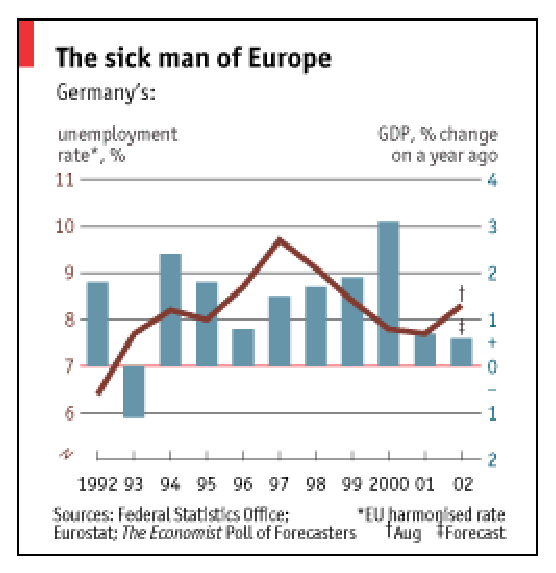
\includegraphics[scale=.4]{sick_man.eps}
  \end{figure}
\end{frame}
%--------------------------------------

%--------------------------------------
\begin{frame}
  \begin{figure}
    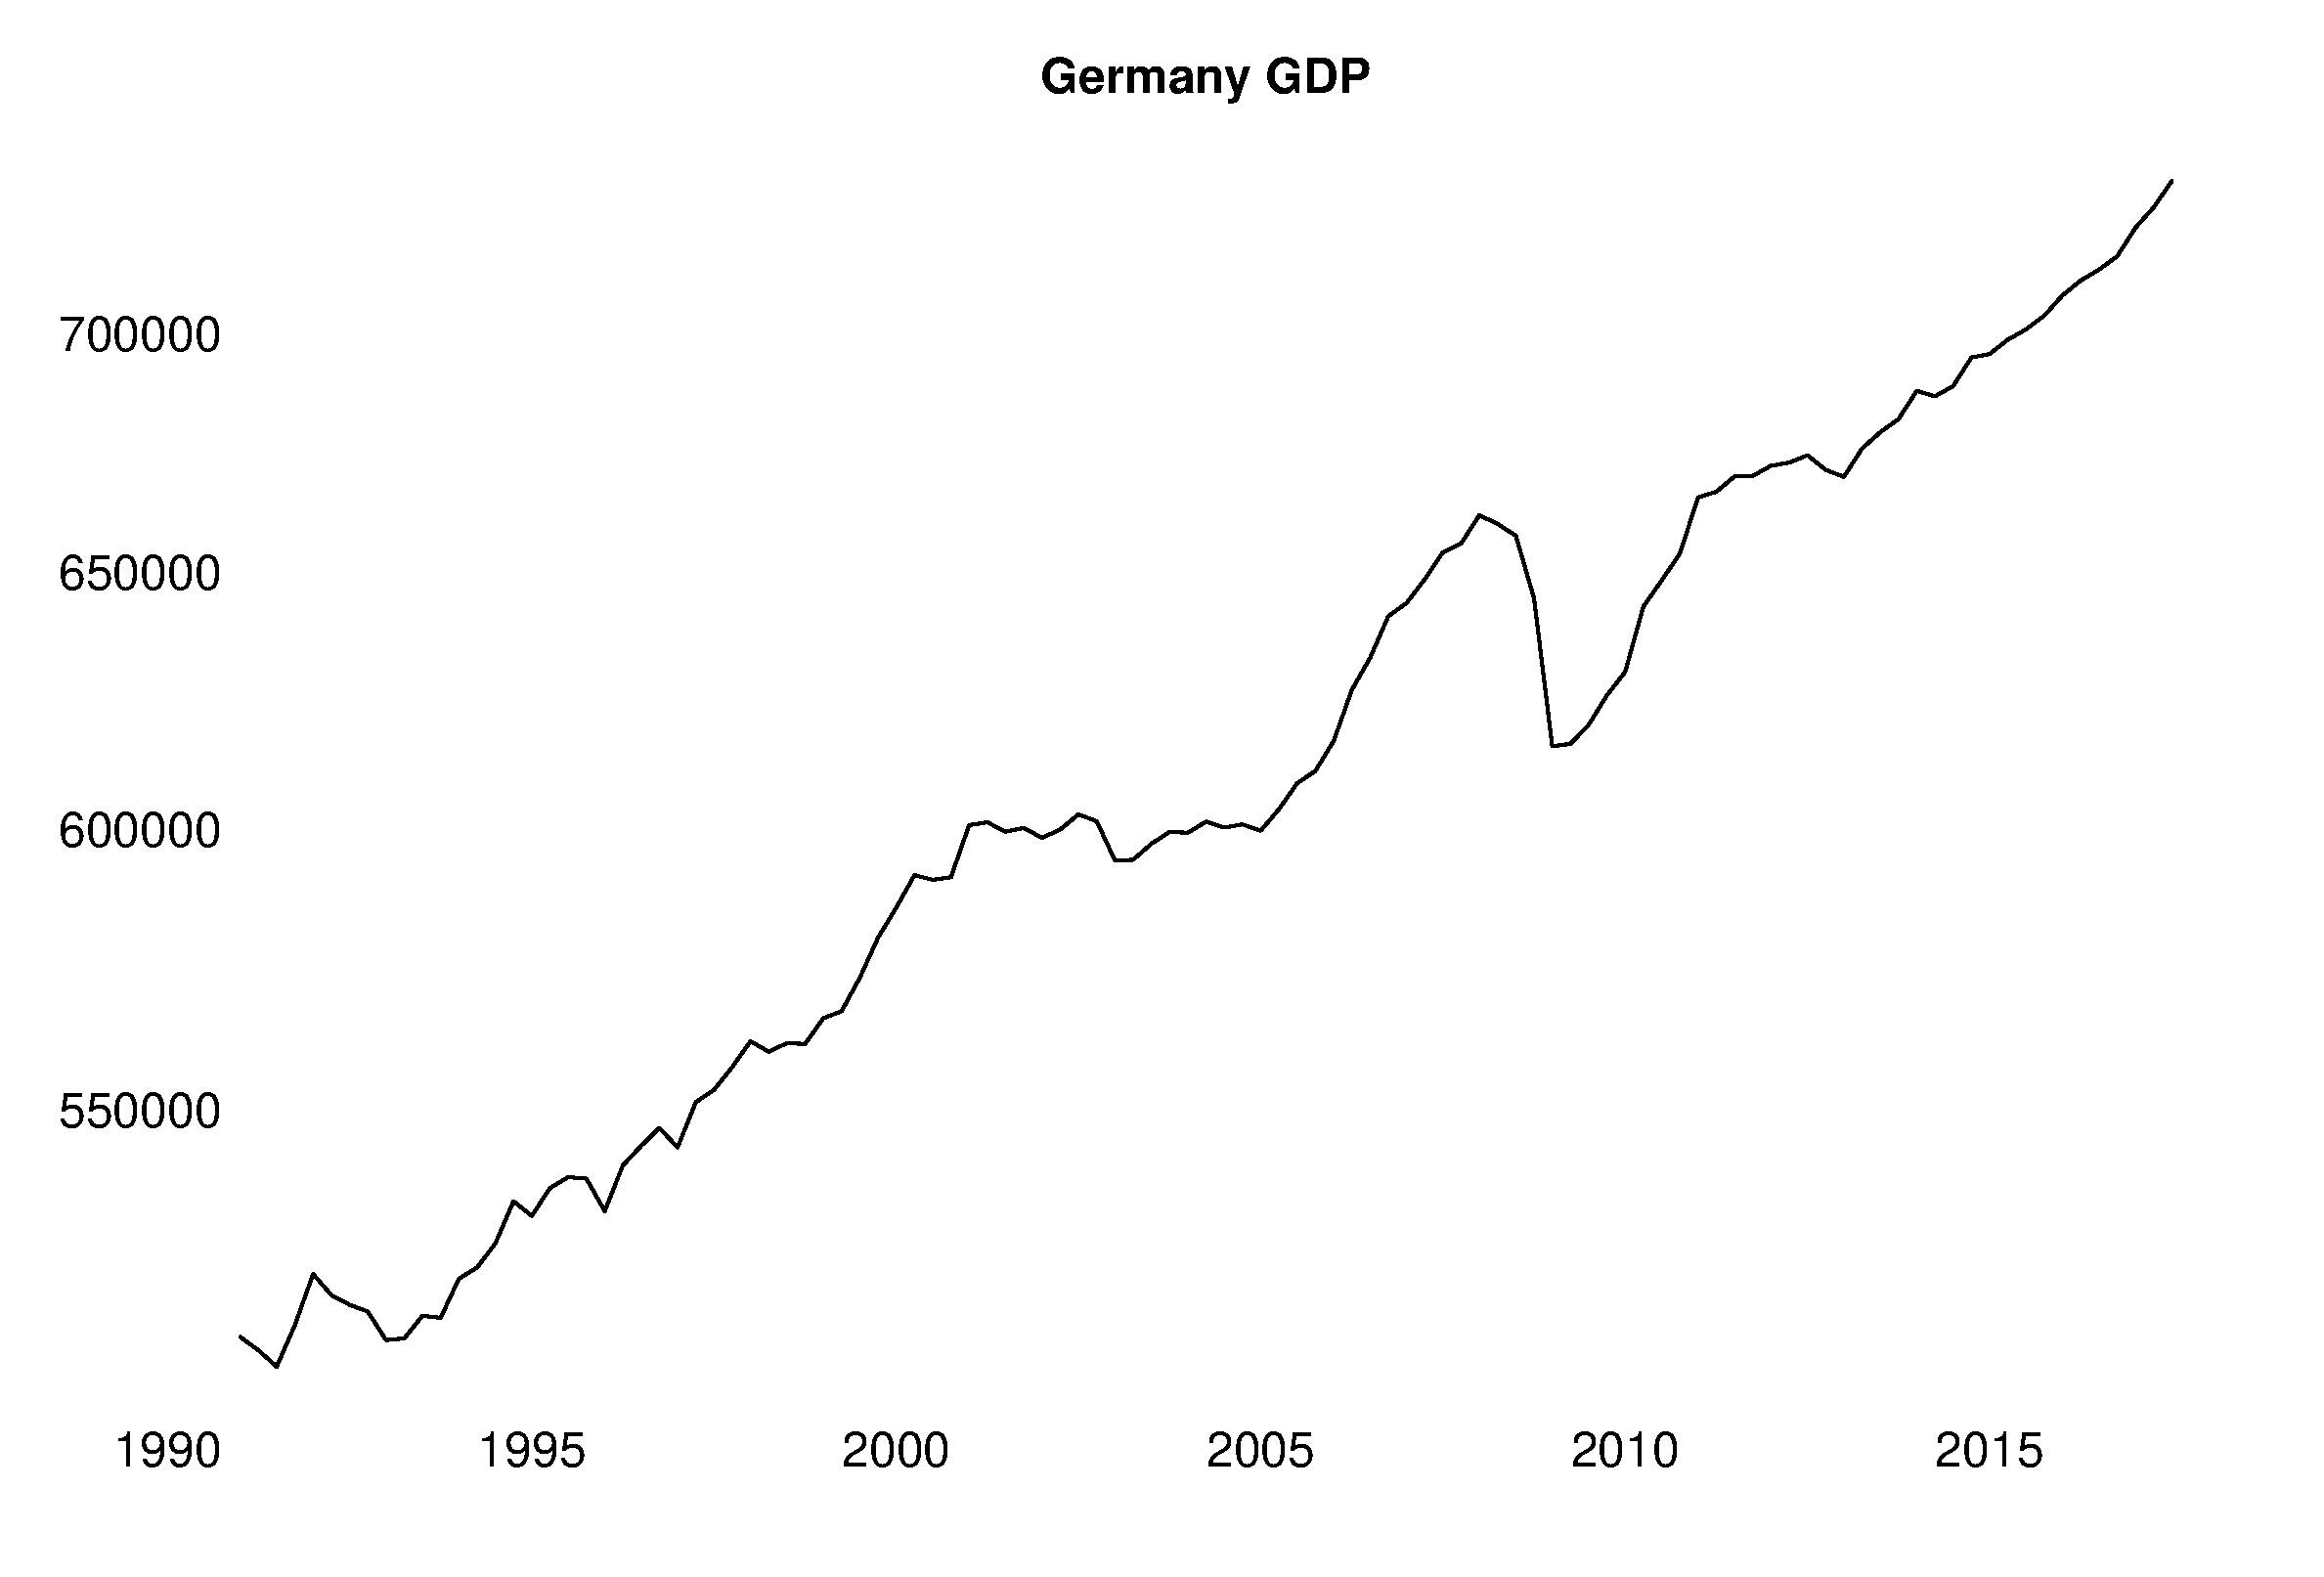
\includegraphics[scale=.3]{germany_gdp.eps}
  \end{figure}
\end{frame}
%--------------------------------------

%--------------------------------------
\begin{frame}
  \textbf{Asymmetric shocks}\\
  \medskip
  Countries will face different shocks when they have different characteristics
  \begin{itemize}
    \item e.g. Germany is not as earthquake-prone as Italy
  \end{itemize}
  \medskip
   Common in OCA: exchange rate  
  \begin{itemize}
    \item Faced with asymmetric shock, central bank has to make a decision
    \item Decision will likely have diverging effects: common exchange rate cannot insulate all countries
  \end{itemize}
\end{frame}
%--------------------------------------

%--------------------------------------
\begin{frame}
  \textbf{Symmetric shocks with asymmetric effects}\\
  \medskip
  Countries experience same shock but react differently
  \begin{itemize}
    \item Result of socio-economic structure: labour regulations, external debt, etc.
  \end{itemize}
  \medskip
  Consider fall out of Brexit
  \begin{itemize}
    \item Ireland and Denmark exposed due to trade relations
    \item Poland and Portugal more insulated
  \end{itemize}
\end{frame}
%--------------------------------------

%--------------------------------------
\begin{frame}
  \textbf{Optimum} Currency Area theory might be bit misleading
  \begin{itemize}
    \item Theory does not discuss optimum conditions
    \item Also no discussion on type of countries that should form currency area
  \end{itemize}
  \medskip
  McKinnon \& Kenen expanded OCA theory including some criteria
  \begin{itemize}
    \item These criteria are endogenous
  \end{itemize}
\end{frame}
%--------------------------------------

%--------------------------------------
\begin{frame}
 \textbf{Criteria} for an optimum currency area  
  \begin{enumerate}
    \item Labour mobility
    \item Production diversification
    \item Openness
    \item Fiscal transfers
    \item Homogeneous preferences
    \item Cross-national solidarity
  \end{enumerate}
  \medskip
  \textbf{NB-} there are three economic and three political criteria
\end{frame}
%--------------------------------------

%--------------------------------------
\begin{frame}
  \textbf{Labour mobility} 
  \begin{quote}
    In an OCA the people should be able to move easily between regions
  \end{quote}
  \medskip
  Important mechanism for dealing with shocks  
  \begin{itemize}
    \item When factors of production can move freely shocks can be mitigated more easily
  \end{itemize}
  \medskip
  Various barriers to migration exist of course
  \begin{itemize}
    \item Economic costs
    \item Skill of migrant worker
    \item Cultural factors such as language    
  \end{itemize}
\end{frame}
%--------------------------------------

%--------------------------------------
\begin{frame}
  \textbf{Production diversification}
  \begin{quote}
    Having a similar production structure and widely diversified production and exports is beneficial for a OCA
  \end{quote}
  \medskip
  Main problem for currency areas: asymmetric shocks
  \begin{itemize}
    \item How often do these shocks occur?
    \item If shocks are rare: costs will be episodic; profits accrue every day    
  \end{itemize}
  \medskip
    Specialised economies are more severely affected by shocks
  \begin{itemize}
    \item $Pr(\sigma_a)$ reduced if countries produce similar goods in diversified economy
    \item Not clear how diversified economies should be
  \end{itemize}
\end{frame}
%--------------------------------------

%--------------------------------------
\begin{frame}
  \textbf{Openness} 
  \begin{quote}
    When countries are open to trade and trade heavily with each other, they could form an OCA
  \end{quote}
  \medskip
   OCA has no distinction between domestic and foreign good 
  \begin{itemize}
    \item Similar to free trade situation
    \item Competition will lead to price equalisation, for most goods, when expressed in same currency
    \item Exchange rate changes affect competitiveness through exports
    \begin{itemize}
      \item Firm more export oriented at certain price levels as it is more profitable
    \end{itemize}    
  \end{itemize}
\end{frame}
%--------------------------------------


%--------------------------------------
\begin{frame}
  \textbf{Fiscal transfers} 
  \begin{quote}
    When countries agree to compensate each other for adverse shocks, they form an OCA
  \end{quote}
  \medskip
   This entails a \textbf{moral hazard} issue  
  \begin{itemize}
    \item Countries might be expecting transfers to happen; lead to slacking
    \item e.g. no diversified economy; heavy import dependence; rigid labour markets
  \end{itemize}
  \medskip
  Free-riding behaviour important discourse during eurocrisis
  \begin{itemize}
    \item North/south antagonism
  \end{itemize}
\end{frame}
%--------------------------------------

%--------------------------------------
\begin{frame}
  \textbf{Homogeneous preferences}
  \begin{quote}
    Currency union member countries must reach consensus on the best way to deal with shocks
  \end{quote}
    \medskip
  \textbf{Solidarity vs. nationalism}\\
   Common monetary policy might give rise to conflicts of national interests
  \begin{itemize}
    \item Costs need to be accepted for the greater good 
    \item Acceptable when
    \begin{align*}
      Costs < \sum Benefits
    \end{align*}    
  \end{itemize}
  Criteria implies move to political union at some time in the future  
\end{frame}
%--------------------------------------

%--------------------------------------
\begin{frame}
  \textbf{Labour mobility} important mechanism to deal with asymmetric shocks: but there are obstacles
  \medskip
\begin{itemize}
  \item Cost of moving 
  \item Risk of becoming unemployed in the destination country
  \item Family prospects
  \item Fiscal factors: social benefits, taxation on earnings, etc.
\end{itemize}
\end{frame}
%--------------------------------------

%--------------------------------------
\begin{frame}
  Other factors influencing migration decision include  
  \begin{itemize}
    \item Cultural differences
    \item Links with family and friends
    \item Commitment to origin country
  \end{itemize}
  \medskip
  Combination of factors means that migration will be limited
\end{frame}
%-------------------------------------


%--------------------------------------
\begin{frame} 
  Compare US with European labour mobility  
  \begin{itemize}
    \item Similar geographic size
    \item Same level of economic development
    \item Comparable within-area differences: Greece is Europe's Mississippi
  \end{itemize}
\end{frame}
%--------------------------------------

%--------------------------------------
\begin{frame}
  \begin{figure}
    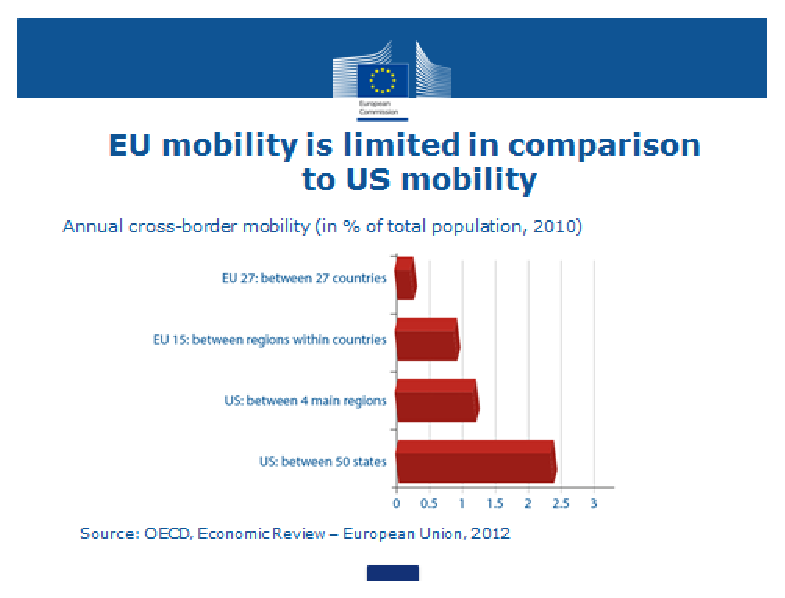
\includegraphics[scale=.7]{eu_labour.eps}
  \end{figure}
\end{frame}
%--------------------------------------

%--------------------------------------
\begin{frame}
  \begin{figure}
    
\includegraphics[scale=.7]{eu_labour2.eps}
  \end{figure}
\end{frame}
%--------------------------------------

%--------------------------------------
\begin{frame}
  \begin{figure}
    
\includegraphics[scale=.7]{eu_labour3.eps}
  \end{figure}
\end{frame}
%--------------------------------------

%--------------------------------------
\begin{frame}
  \begin{figure}
    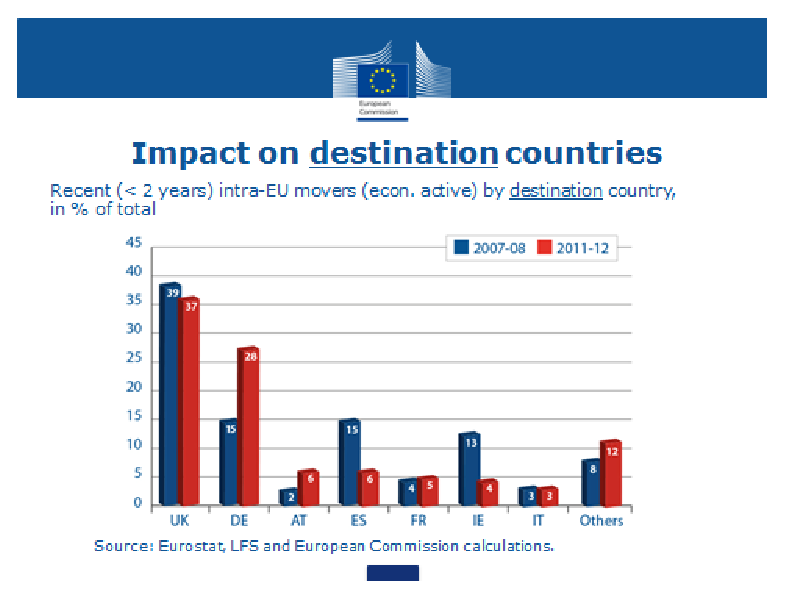
\includegraphics[scale=.7]{eu_labour4.eps}
  \end{figure}
\end{frame}
%--------------------------------------

%--------------------------------------
\begin{frame}
  High unemployment levels associated with adverse asymmetric shocks
  \begin{itemize}
    \item Specifically given low labour moblity levels in EU
  \end{itemize}
  \medskip
  Important that economies are 
  \begin{enumerate}
    \item Diversified
    \item Open to trade
  \end{enumerate}
  \medskip 
  Frequency of asymmetric shocks is lower among countries with
  \begin{itemize}
    \item Similar production patterns
    \item Diversified trade pattern
  \end{itemize}
\end{frame}
%--------------------------------------

%--------------------------------------
\begin{frame}
  \begin{figure}
    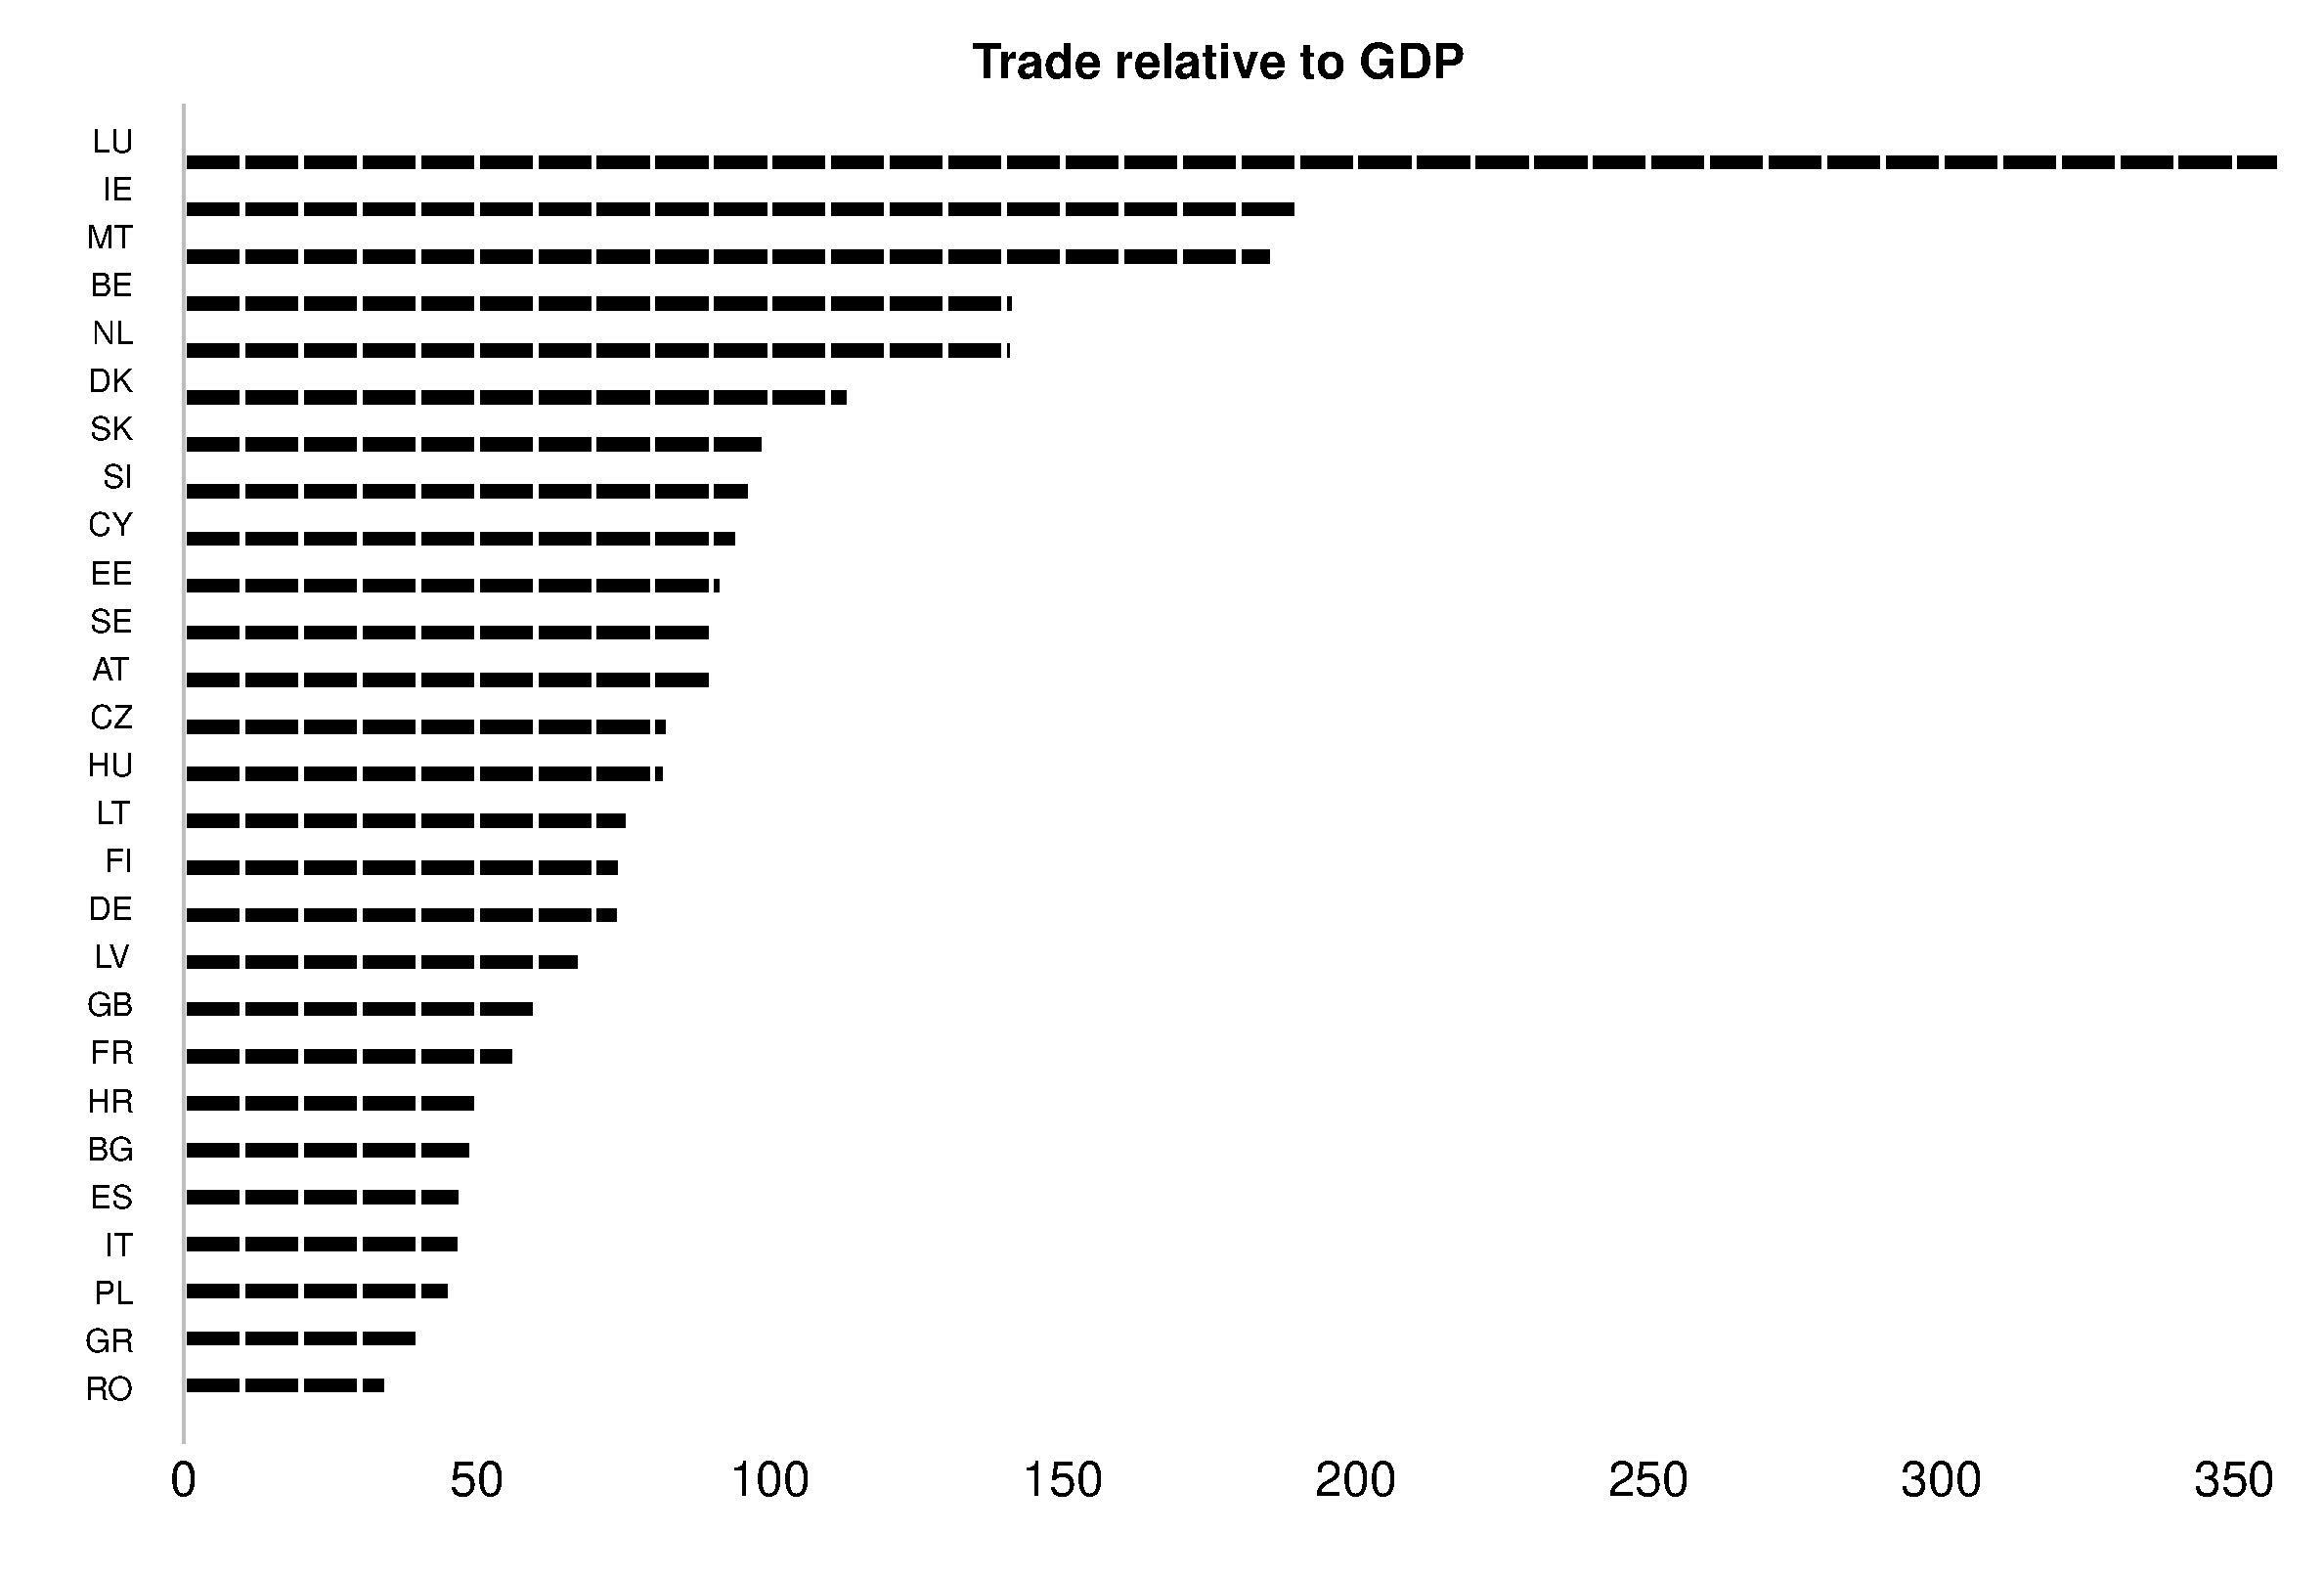
\includegraphics[scale=.3]{openness.eps}
  \end{figure}
\end{frame}
%--------------------------------------


%--------------------------------------
\begin{frame}
  \textbf{Homogeneous preferences} on monetary and fiscal policy is an import economic criteria. 
  \begin{itemize}
    \item Monetary policy is an important tool dealing with shocks
    \item Fiscal policy important with regard to public debt
  \end{itemize}
  \medskip
   For homogeneity can look at long term trends:  
  \begin{enumerate}
    \item Inflation rate: for monetary policy
    \item Public debt levels: for fiscal policy
  \end{enumerate}
\end{frame}
%--------------------------------------


%--------------------------------------
\begin{frame}
  \begin{figure}
    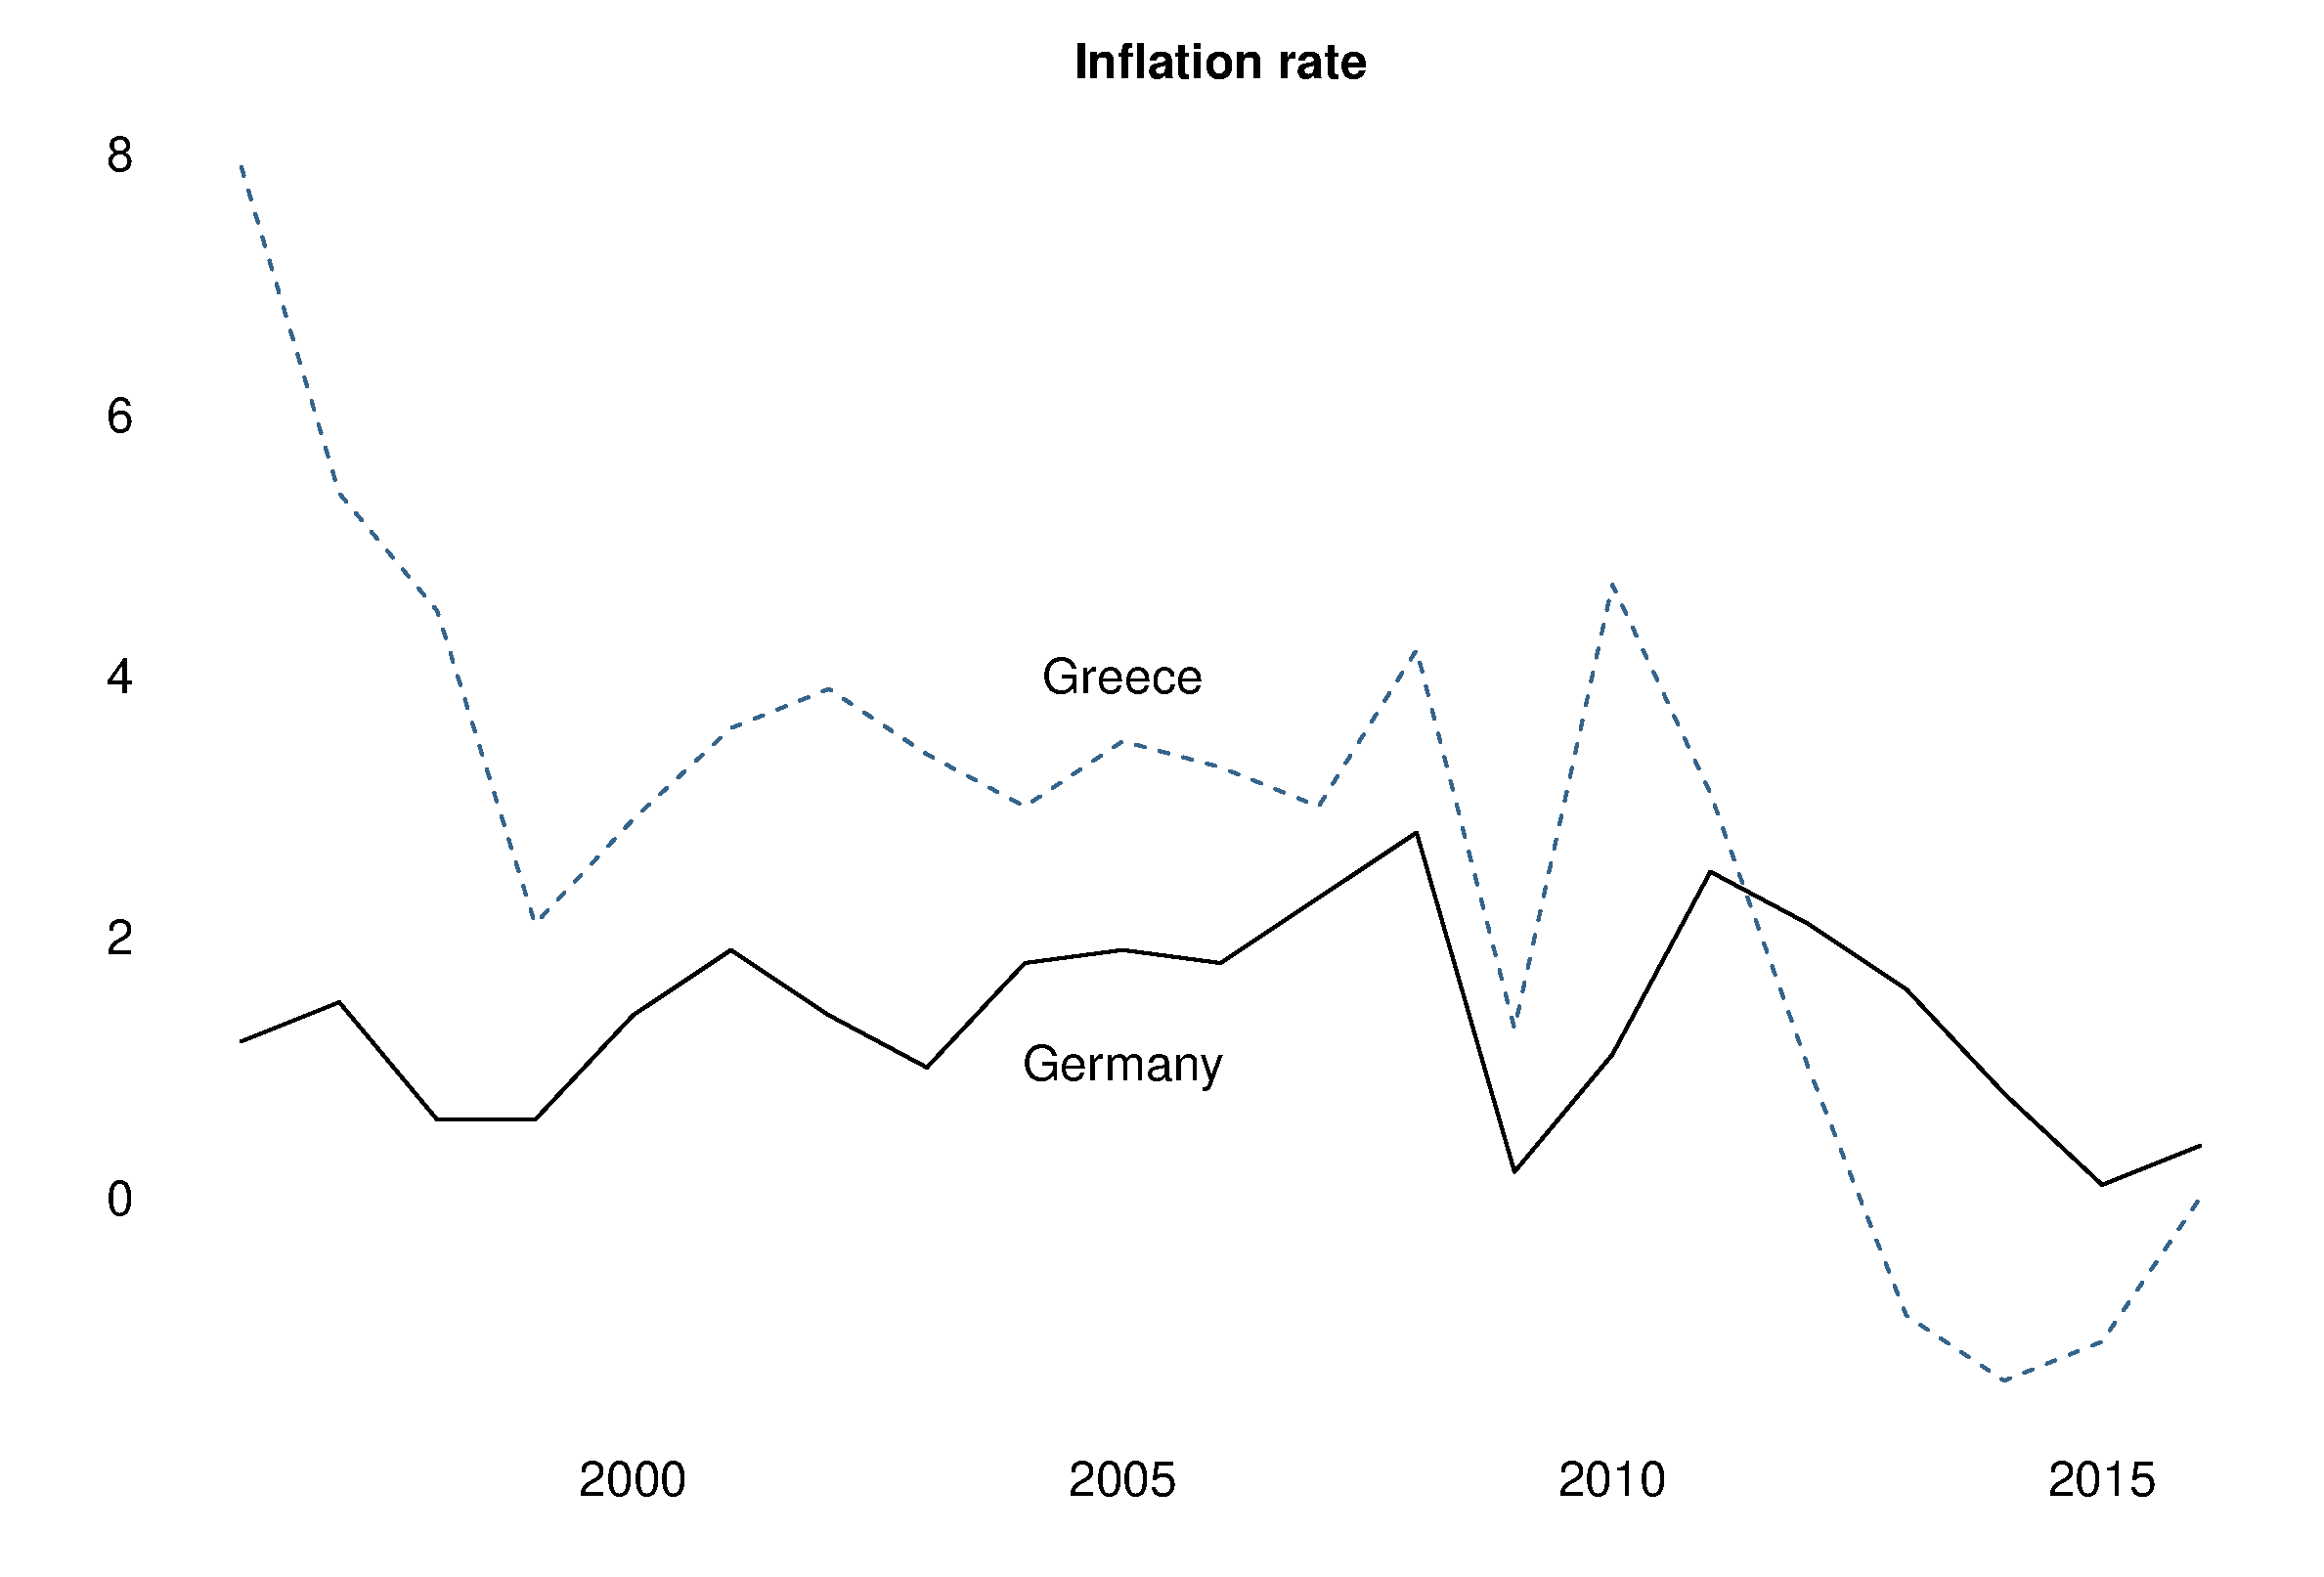
\includegraphics[scale=.3]{inflation.eps}
  \end{figure}
\end{frame}
%--------------------------------------

%--------------------------------------
\begin{frame}
  \begin{figure}
    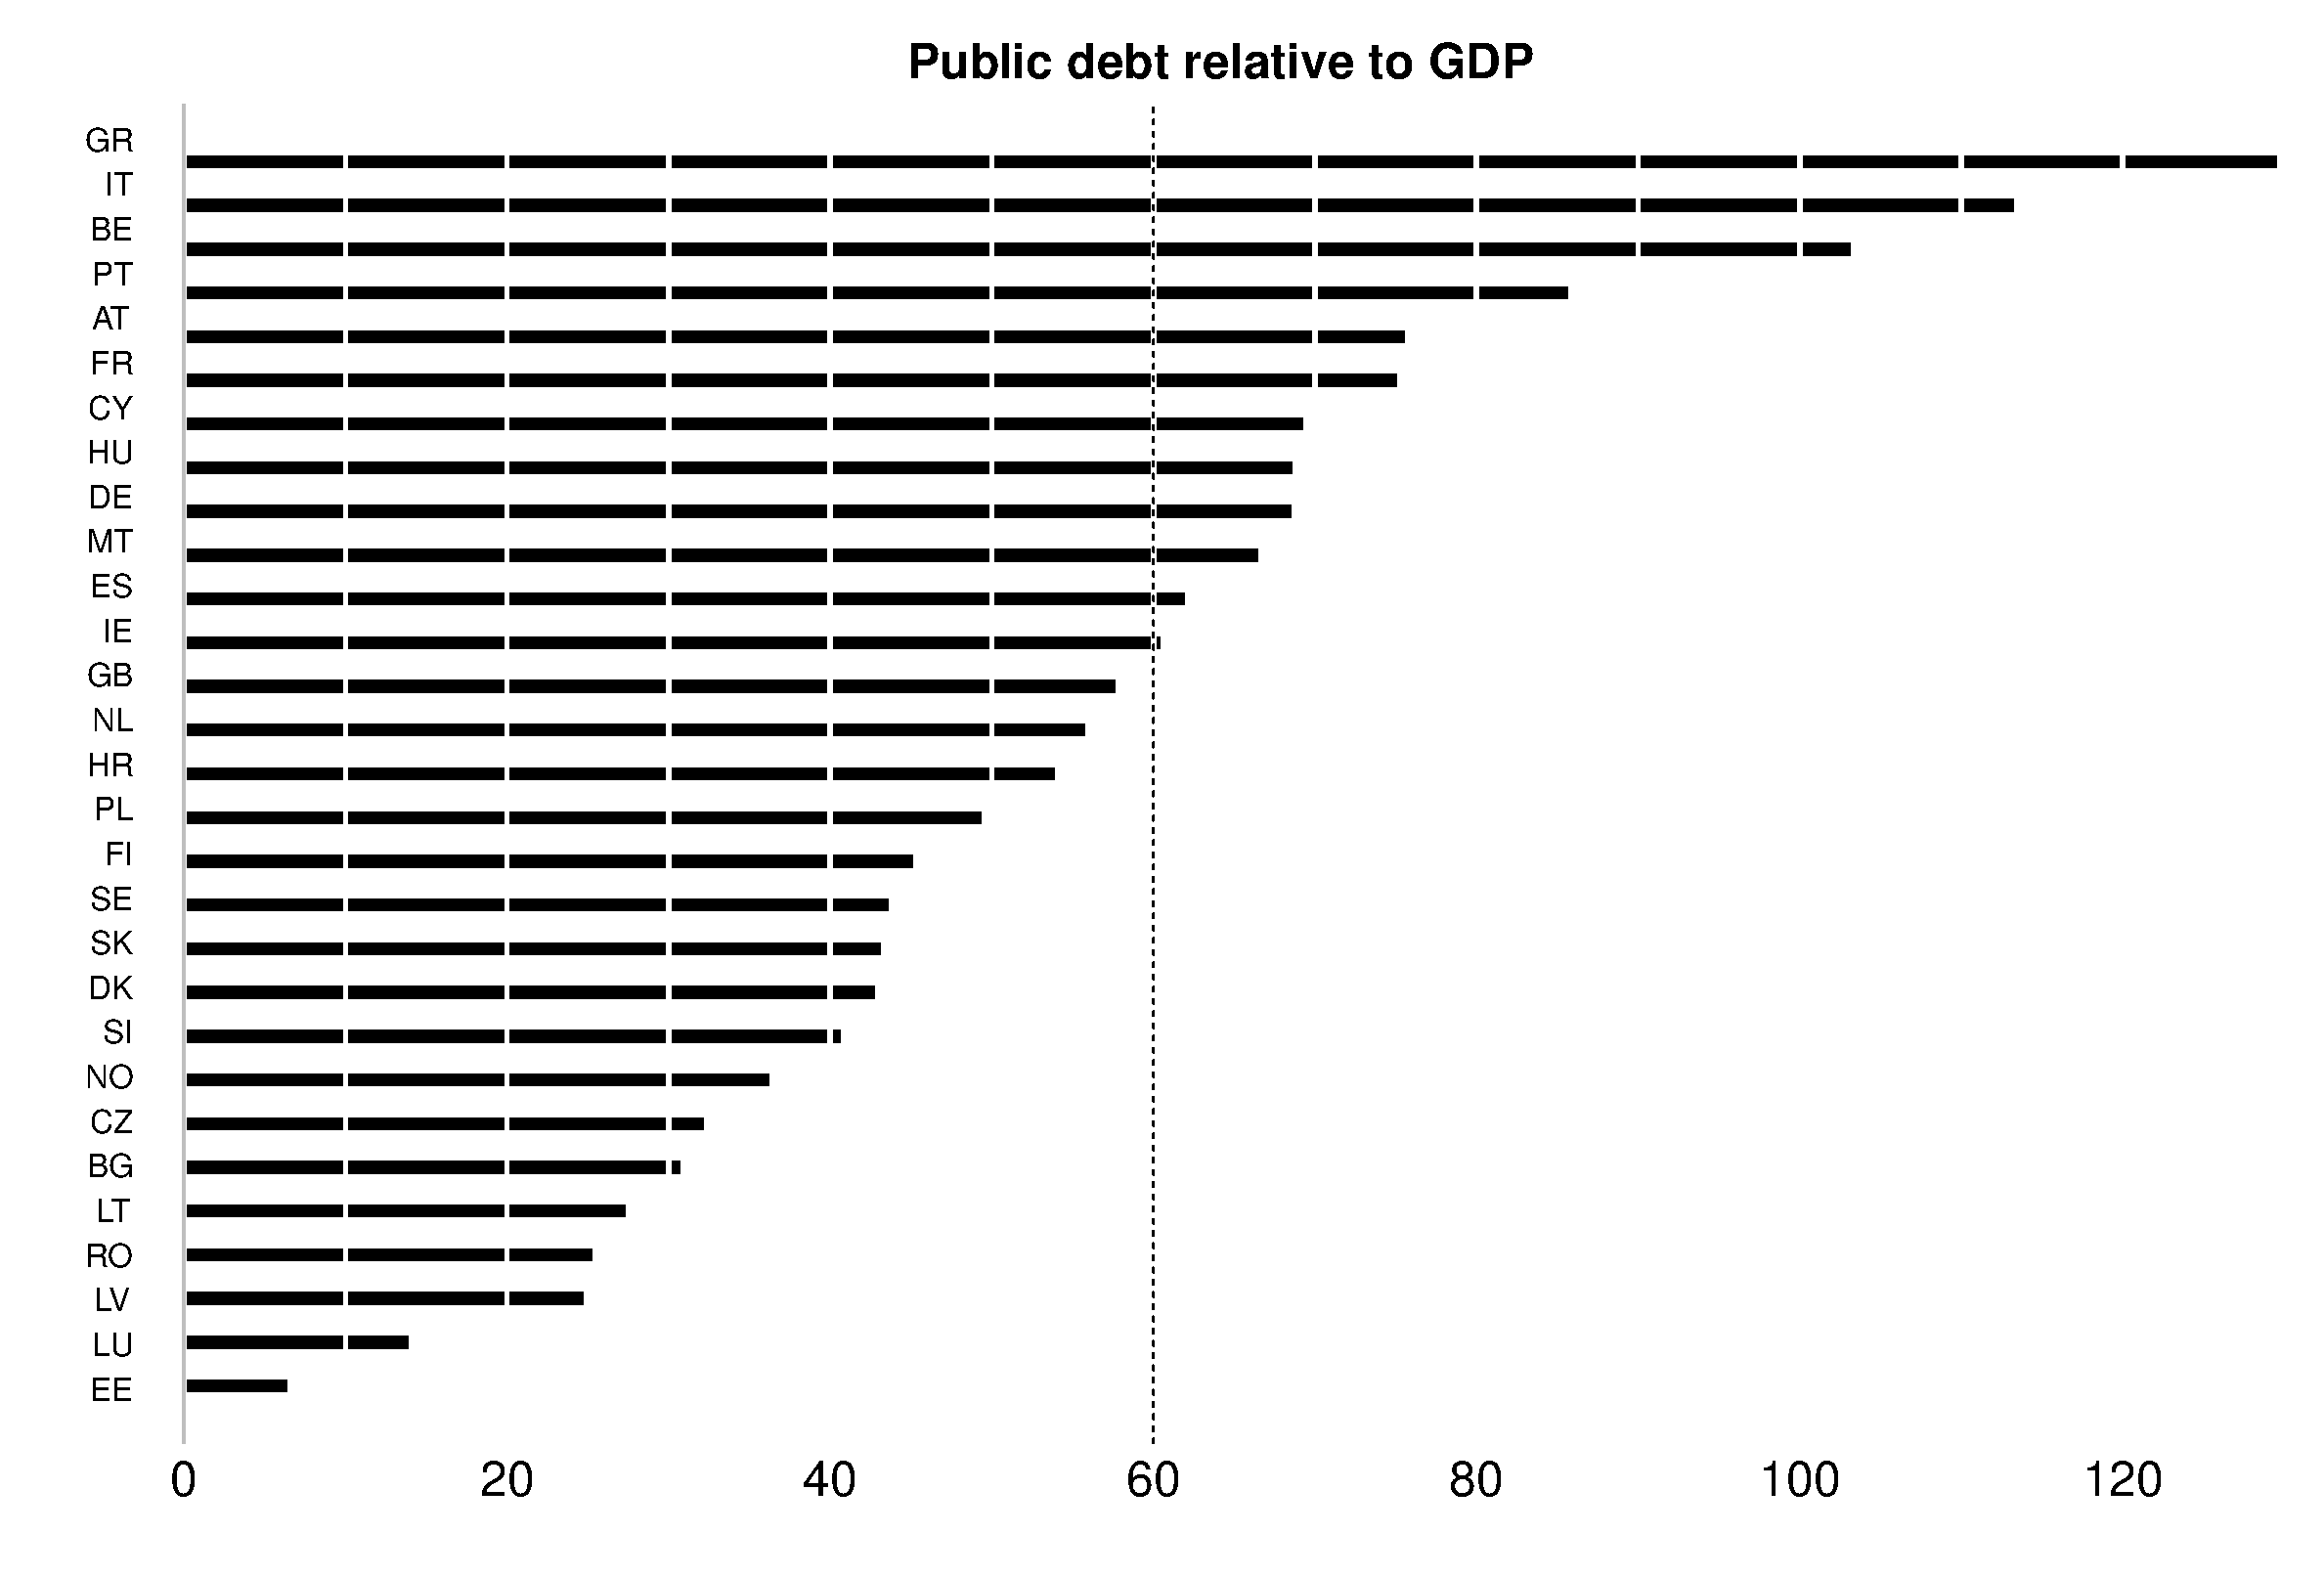
\includegraphics[scale=.3]{public_debt.eps}
  \end{figure}
\end{frame}
%--------------------------------------

%--------------------------------------
\begin{frame}
  What explains differences in macroeconomic policy across countries?
  \begin{itemize}
    \item Politician's incentives; shapes national institutions
    \item e.g. strong labour union movements; emphasis on public goods provision
  \end{itemize}  
\end{frame}
%--------------------------------------

%--------------------------------------
\begin{frame}
  \textbf{Common institutions} can help homogenise policy, e.g. European Central Bank
  \begin{itemize}
    \item ECB determines monetary policy for eurozone
    \item Main objective: price stability
  \end{itemize}
  \medskip
  All national budget are subject to \textbf{excessive debt procedure}   
  \begin{itemize}
    \item Aimed at curtailing excessive public spending
    \item Operation under common institutions does not imply agreement on best course of action in dealing with shocks
  \end{itemize}
\end{frame}
%--------------------------------------


%--------------------------------------
\begin{frame}
  \textbf{Fiscal transfers}: let's check EU budget
  \begin{enumerate}
    \item Structural fund and Cohesion policy (50\%)
    \item Common Agricultural Policy (43\%)
    \item Operating expenses (6\%)
  \end{enumerate}
  \medskip
  In general the budget of the European Union is very small at about only 1\% of the combined GDP of all EU member states. 
\end{frame}
%--------------------------------------

%--------------------------------------
\begin{frame}
 No cyclical transfer system in EU/eurozone  
  \begin{itemize}
    \item Structural fund/Cohesion policy transfers money to assist in stimulating economy in long-run
    \item EU regions with a GDP below 75\% of the EU average; regardless of shocks
    \item Transfers are for 7-year period and not cyclical
  \end{itemize}
\end{frame}
%--------------------------------------

%--------------------------------------
\begin{frame}
 \textbf{European Stability Mechanism} (ESM) is an important first step towards fiscal transfers
   \begin{itemize}
    \item Established following the eurocrisis (2012)
    \item ESM member states can apply for ESM bailout when 
    \begin{enumerate}
      \item They are in serious financial difficulty
      \item Their banks need recapitalisation. 
    \end{enumerate}
  \end{itemize}       
\end{frame}
%--------------------------------------


%--------------------------------------
\begin{frame}
  \begin{figure}
    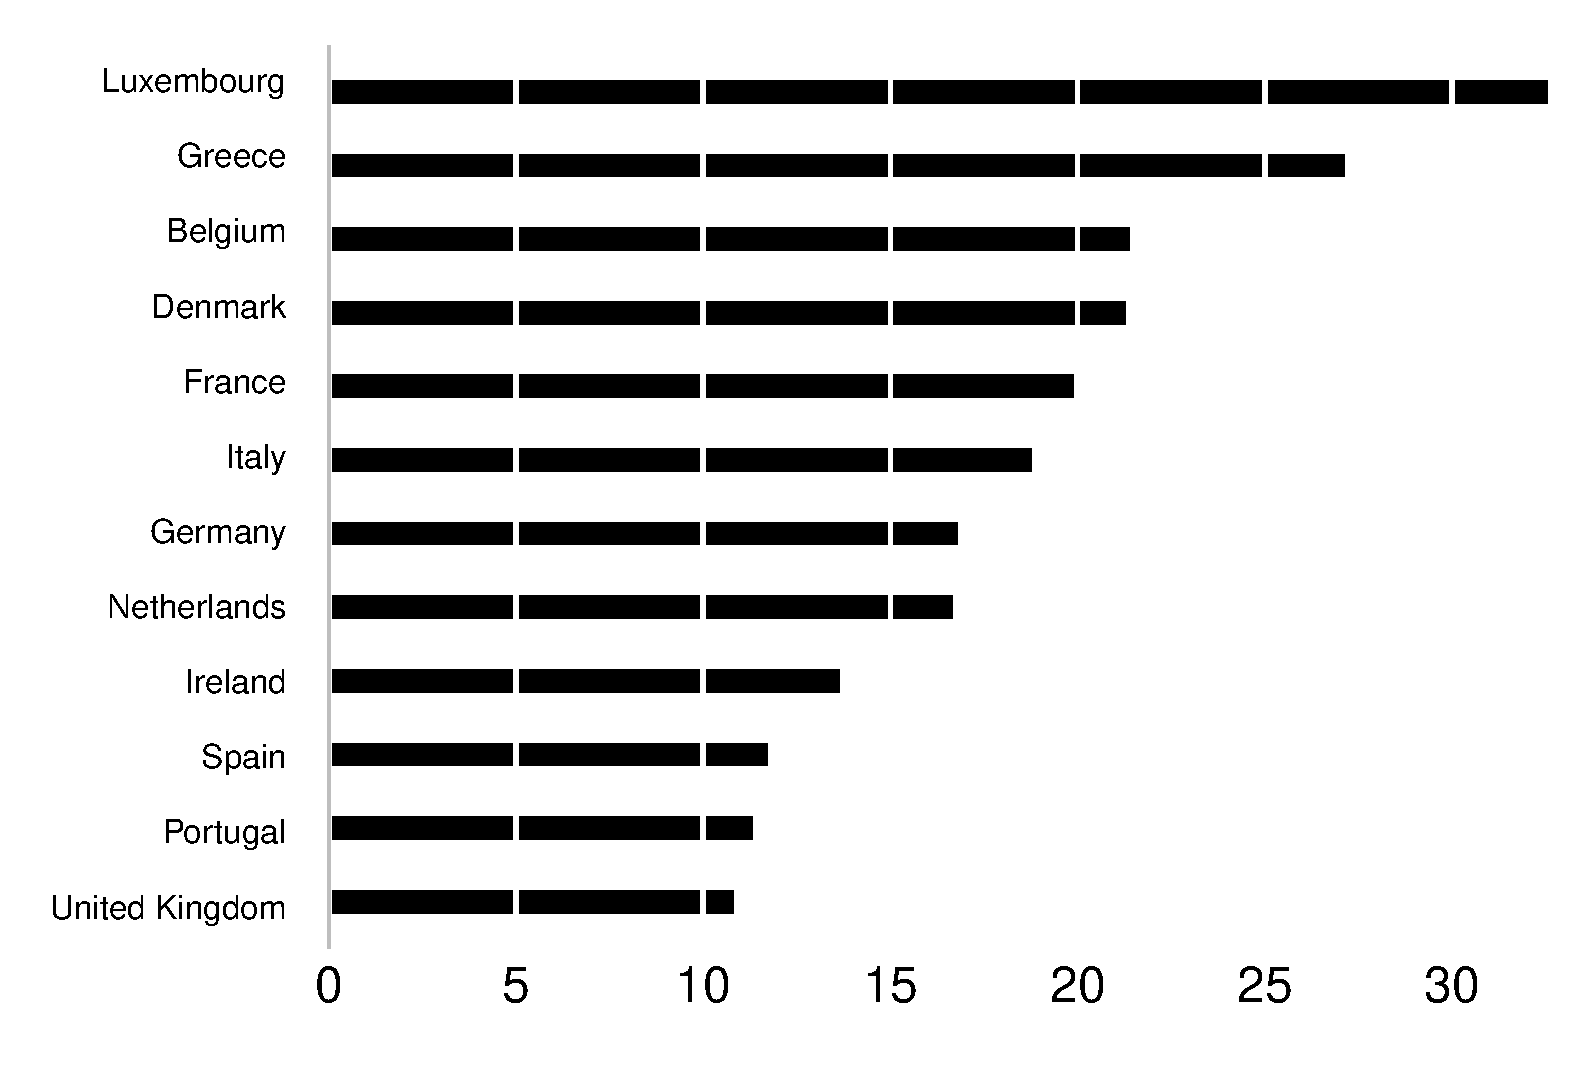
\includegraphics[scale=.4]{eurobarometer.eps}
  \end{figure}
\end{frame}
%--------------------------------------

%--------------------------------------
\begin{frame}
  \textbf{Euroskepticism}
  \begin{itemize}
    \item EU constitution rejection by French and Dutch voters (2005)
    \item Nativist movements following Great Recession (FRA, NLD, AUT, GER, GRC, ITA) 
    \item Brexit (2016)
    \item Poland, Hungary
  \end{itemize}
  \medskip
  More enthusiasm for European project can be found in   
  \begin{itemize}
    \item Scotland, Catalonia
    \item Ukraine, Georgia
  \end{itemize}
\end{frame}
%--------------------------------------

%--------------------------------------
\begin{frame}
\begin{table}[!h] \centering \caption{Scorecard for the OCA criteria} \label{table:summary}
\scalebox{1}{\begin{tabular}{lc}
\\[-1.8ex]\hline 
\hline \\[-1.8ex] 
Criterion & Satisfied\\
\hline \\[-1.8ex]\\
Labour mobility & No\\
Trade openness  & Yes\\
Product diversification & Yes\\
Fiscal transfers & No\\
Homogeneous preferences & Partially\\
Commonality of destiny & Hard to tell\\
    \\[-1.8ex]\hline 
    \hline \\[-1.8ex]
\end{tabular} }  
\end{table}
\end{frame}
%--------------------------------------

%--------------------------------------
\begin{frame}
  \begin{enumerate}
  \item Euro project remains controversial
  \begin{itemize}
    \item Difficult to make hard case for either stance 
    \item OCA criteria more guiding principle rather than iron law
    \item Decision for monetary union ultimately rests on political considerations
  \end{itemize}
  \medskip
  \item Proceeding entails future costs; given partial fulfillment OCA criteria  
  \begin{itemize}
    \item Costs will mainly arise in labour market and fiscal transfers
    \item Eurozone crisis showed that asymmetric shocks happen and can be painful
  \end{itemize}
\end{enumerate}
\end{frame}
%--------------------------------------

%--------------------------------------
\end{document}
